\documentclass[oneside,final,11pt]{article}
\usepackage[utf8]{inputenc}
\usepackage[russianb]{babel}
\usepackage{vmargin}
\usepackage{amsmath}
\usepackage{amsfonts}
\usepackage{amssymb}
\usepackage{amsthm}
\usepackage[matrix,arrow,curve]{xy}
\usepackage{graphicx}
\setpapersize{A4}
\setmarginsrb{2cm}{1.5cm}{1cm}{1.5cm}{0pt}{0mm}{0pt}{13mm}
\usepackage{indentfirst}
\sloppy

\DeclareMathOperator{\conv}{conv}

\newcommand*\Rn  [1]{\mathbb{R}^{#1}}
\newcommand*\Rnn[1]{\mathbb{R}^{#1 \times #1}}
\newcommand*\Chi {\mathcal{X}}
\newcommand*\Pset{\mathcal{P}}
\newcommand*\Sset{\mathcal{S}_1(0)}
\renewcommand*\leq{\leqslant}

\newcommand*\norm[2]{\|#1\|_{#2}}
\newcommand*\segm[2]{[#1,#2]}
\newcommand*\scprod[2]{\bigl\langle #1 , #2 \bigl\rangle}
\newcommand*\spfun[2]{\rho \bigl( #1 , #2 \bigr)}

\newcommand*\confAB[8]{A(t) = \left(\begin{matrix} #1 & #2 \\ #3 & #4 \\ \end{matrix}\right),\: B(t) = \left(\begin{matrix} #5 & #6 \\ #7 & #8 \\ \end{matrix}\right),\:}
\newcommand*\conffalphar[8]{f(t) = \left(\begin{matrix} #1 \\ #2 \end{matrix}\right) \quad \text{в \eqref{ltp}, и}\\ \alpha = #3,\beta = #4,a = #5, b = #6, c = #7;\: r =#8; \:}
\newcommand*\confq[8]{(q_1, q_2, q_3, q_4) = \left(\left(\begin{matrix} #1 \\ #2  \end{matrix}\right), \left(\begin{matrix} #3 \\ #4 \end{matrix}\right), \left(\begin{matrix} #5 \\ #6 \end{matrix}\right), \left(\begin{matrix} #7 \\ #8 \end{matrix}\right) \right) \quad \text{в \eqref{sets}.}}

\newtheorem*{theorem}{Теорема}
\newtheorem*{remark}{Замечание}

\begin{document}
	\begin{titlepage}
		\begin{centering}
			
\includegraphics[width=0.5\textwidth]{msu.png}\\
			{\scshape Московский государственный университет имени М.~В.~Ломоносова}\\
			Факультет вычислительной математики и кибернетики\\
			Кафедра системного анализа\\
			\vfill
			{\LARGE Лабораторная работа №1}\\
			\vspace{1cm}
			{\Huge\bfseries "<Линейная задача быстродействия">\\}
		\end{centering}
		\vspace{1cm}
		\begin{flushright}
			\begin{large}
				{\itshape Студент 315 группы\\}
				А.~А.~Владимиров\\
				\vspace{5mm}
				{\itshape Руководитель Практикума\\}
				к.ф.-м.н., доцент П.~А.~Точилин\\
			\end{large}
		\end{flushright}
		\vfill
		\begin{centering}
			Москва, 2021\\ 
		\end{centering}
	\newpage
	\end{titlepage}
	\setcounter{page}{2}
	
	\tableofcontents

	\newpage
	\section{Постановка задачи}
		Требуется решить линейную задачу быстродействия:
		\begin{equation} \begin{aligned} \label{ltp}
			&\dot x = A(t)x + B(t)u +f(t), \: t \in [t_0, t_1];\\ 
			&x \in \Rn{2},\: u \in \Pset(t) \text{~--- компактное подмножество }\Rn{2};\\
			&x(t_0) \in  \Chi_0, \: x(t_1) \in \Chi_1;\\
			&t_1 - t_0 \rightarrow \min_{u\scriptscriptstyle{(\cdot)}}.
		\end{aligned} \end{equation} 
		То есть необходимо найти минимальное время \(t^*>0\), за которое траектория системы, выпущенная в момент времени \(t_0\) из некоторой точки множества \(\Chi_0\), может попасть в некоторую точку множества \(\Chi_1\). Конкретно в нашей задаче также известен вид множеств:
		\begin{equation}\begin{aligned}  \label{sets}
			\Pset(t) \equiv\: &\Pset  = \{(x_1,x_2) \in \Rn{2} : \alpha(x_1-a)^2 + \beta(x_2-b)^2 \leq c\},\quad \alpha,\beta,c > 0;\\
			&\Chi_0 = \{(x_1,x_2) \in \Rn{2} : x_1^2 + x_2^2 \leq r^2\},\quad r > 0;\\
			&\Chi_1 =\conv\{q_1,q_2,q_3,q_4\}, \quad q_1,q_2,q_3,q_4 \in \Rn{2}.\\
		\end{aligned}\end{equation}

	\section{Теоретические выкладки}
		Для решения поставленной задачи нам потребуется известная
		\begin{theorem}[ПМП для линейной задачи быстродействия]
			Пусть \((x^*(t),\,u^*(t))\)~--- оптимальная пара в задаче \eqref{ltp}, тогда 
			\begin{gather}
				\exists\:\psi(t) \in \Rn{2} \text{~--- сопряженная переменная}: \notag\\
				\dot \psi(t) = -A^*(t)\cdot\psi(t),\: \psi(t) \ne 0, \label{conjCp}
			\end{gather}
причем имеют место
			\begin{description}
				\item[\mdseries\itshape 1) принцип максимума]
					\begin{equation} \label{pm} 
					\scprod{\psi(t)}{B(t)u^*(t)} \stackrel{\text{п.в}} =  \spfun{\psi(t)}{B(t)\Pset(t)},\end{equation}
				\item[\mdseries\itshape 2) условие трансверсальности на левом конце]														\begin{equation} \label{ltrans}
					\scprod{\psi(t_0)}{x^*(t_0)} = \spfun{\psi(t_0)}{\Chi_0}, \end{equation}
				\item[\mdseries\itshape 3) условие трансверсальности на правом конце]
					\begin{equation} \label{rtrans}
					\scprod{-\psi(t_1)}{x^*(t_1)} = \spfun{-\psi(t_1)}{\Chi_1}. \end{equation}
			\end{description}
		\end{theorem}

		Итак пусть \(\psi(t), t \in \segm{t_0}{t^*}\)~--- сопряженная к оптимальной паре \((x^*(t),\,u^*(t))\) переменная. Сперва найдем начальную точку оптимальной траектории \(x^*(t_0)\). Из левого условия трансверсальности \eqref{ltrans} ясно, что \(x^*(t_0)\)~--- опорная точка функции\footnote{здесь и далее словосочетание "опорная точка функции \(\spfun{\psi}{\mathcal{M}}\)"\: означает опорную точку множества \(\mathcal{M}\) в направелнии вектора \(\psi\). Подобное словоупотребление мотивировано тем, что в качестве аргумента \(\psi\) будут встречаться довольно сложные выражения, которые необходимо явно учитывать в вычислениях. В то же время классическое понятие опорная точка множества плохо отражает (во всяком случае не отражает явно) зависимость этой точки от первого аргумента опорной функции.} \(\spfun{\psi(t_0)}{\Chi_0}\). Ивестно, что для \(\Chi_0\) вида \eqref{sets}
		\[\text{опорная точка } x^* =  \frac{r}{\norm{\psi}{2}}\psi,\]
где \(\psi\) ~--- аргумент опорной функции \(\spfun{\psi}{\Chi_0}\).\par
	Не ограничивая общности допустим, что \( \norm{\psi(t_0)}{2} = 1\), тогда
		\begin{equation} \label{initval}
			x^*(t_0) = r\psi(t_0).
		\end{equation}\par
		
		Далее, используя принцип максимума \eqref{pm} получим управление \(u^*(t)\). Обозначим за \(v^*(t)\) опорную точку функции \(\spfun{\psi(t)}{B(t)\mathcal{P}(t)} = \spfun{\psi(t)}{B(t)\Pset}\) для почти всех \(t \in \segm{t_0}{t^*}\). Тогда из \eqref{pm}
		\[u^*(t) = B^{-1}(t)v^*(t).\]
Из определения опорной функции и свойства: \(\spfun{\psi(t)}{B(t)\Pset} = \spfun{B^*(t)\psi(t)}{\Pset}\); очевидно следует, что
			\[v^*(t) = B(t)w^*(t),\]
где \(w^*(t)\) ~--- опорная точка для \(\spfun{B^*(t)\psi(t)}{\Pset}\).\par
	Поскольку
		\begin{gather*}
			\Pset = P\Sset + q,\\
			\text{где }P = \left( \begin{matrix} \sqrt{\alpha c} & 0 \\ 0 & \sqrt{\beta c}\\ \end{matrix} \right),\: q = \left(\begin{matrix} a\\b\\ \end{matrix}\right),\:\Sset =  \{(x_1,x_2) \in \Rn{2} : x_1^2 + x_2^2 \leq 1\} \quad \text{(cм. \eqref{sets}),}
		\end{gather*}
имеем
		\[\spfun{B^*(t)\psi(t)}{\Pset} = \spfun{B^*(t)\psi(t)}{P\Sset + q} = \spfun{P^*B^*(t)\psi(t)}{\Sset} + \spfun{B^*(t)\psi(t)}{q}  = \varrho_1(t) + \varrho_2(t). \]
Опорные точки функций \(\varrho_1(t) + \varrho_2(t)\) известны и равны 
		\[q^*_1(t) = \frac{P^*B^*(t)\psi(t)}{\norm{P^*B^*(t)\psi(t)}{2}},\: q^*_2(t)  = q,\:\text{соответственно.}\]
Возвращаясь к поиску опорной точки \(w^*(t)\) во множестве \(\Pset\) получим
		\[w^*(t) = Pq^*_1(t) + q^*_2(t) = P\frac{P^*B^*(t)\psi(t)}{\norm{P^*B^*(t)\psi(t)}{2}} + q.\]
Наконец, явно выразим искомую точку \(u^*(t)\)
		\begin{equation} \label{optcntrl} \begin{split}
			u^*(t) =  B^{-1}(t)v^*(t) = B^{-1}(t)B(t)w^*(t) = w^*(t) = (Pq^*_1(t) + q^*_2(t)) = \frac{PP^*B^*(t)\psi(t)}{\norm{P^*B^*(t)\psi(t)}{2}} + q,\:\text{где}\\
			P = \left( \begin{matrix} \sqrt{\alpha c} & 0 \\ 0 & \sqrt{\beta c}\\ \end{matrix} \right),\: q = \left(\begin{matrix} a\\b\\ \end{matrix}\right);\: B(t) \text{~--- некоторая заданная матрица.}
		\end {split} \end{equation}

Таким образом, располагая соответсвующей сопряженной переменной \(\psi(t), t \in \segm{t_0}{t^*}\) не состовляет труда получить \eqref{initval}, \eqref{optcntrl} начальную точку \(x^*(t_0)\) и оптимальное управление \(u^*(t), t \in \segm{t_0}{t^*}\). Подставляя полученные значения в \eqref{ltp} получим классическую задачу Коши, при соблюдении условий гладкости имеющюю единственное решение~--- оптимальную траекторию \(x^*(t), t \in \segm{t_0}{t^*}\), где \(t^*\)~--- минимальное время. Более того, для получения траектории сопряженной переменной \(\psi(t)\) достаточно иметь начальное условие \(\psi(t_0)\) и решить соответствующую задачу Коши \eqref{conjCp}.
		{\theoremstyle{plain} \begin{remark}
			 Остались не обсужденными проблемы нахождения {\bfseries оптимальных} \(\psi(t_0)\) и \(t^*\). Первая из них решается банальным перебором (осуществляемым, разумеется, компьютером), хоть и немного оптимизированным: ввиду свойств опорных функций мы можем, не сужая множество получаемых на выходе управлений и начальных точек траекторий, подозрительных на оптимальность, перебирать лишь нормированные \(\psi(t_0)\), т.е лежащие на единичной окружности.  С нахождением \(t^*\) все немного сложнее. Потребуется для каждого перебираемого значения \(\psi(t_0)\), по достижении целевого множества (или при выходе за некоторое предельно допустимое время), останавливать процесс интегрирования соответствующей задачи Коши \eqref{ltp}. После осуществления перебора выбрать наименьшее \(t^*_{min}\). Соответствующие \(t^*_{min}\) управление и траекторию будем считать приближенно оптимальными. Точность полученного приближения можно оценить сравнив значения правой и левой части правого условия трансверсальности \eqref{rtrans}. 
		\end{remark}}

	\section{Примеры}
		Ниже приведены иллюстрации найденных алгоритмом решений для некотрых конфигураций системы.
		
		\newpage
		\subsection{автономная система}
			\begin{gather*}
				\confAB{2}{2}{3}{0}{1}{6}{20}{3}
				\conffalphar{8}{7}{1}{2}{0.5}{3}{2}{3}
				\confq{10}{10}{10}{15}{15}{10}{15}{15}
			\end{gather*}
			\begin{figure}[h]
				\centering
				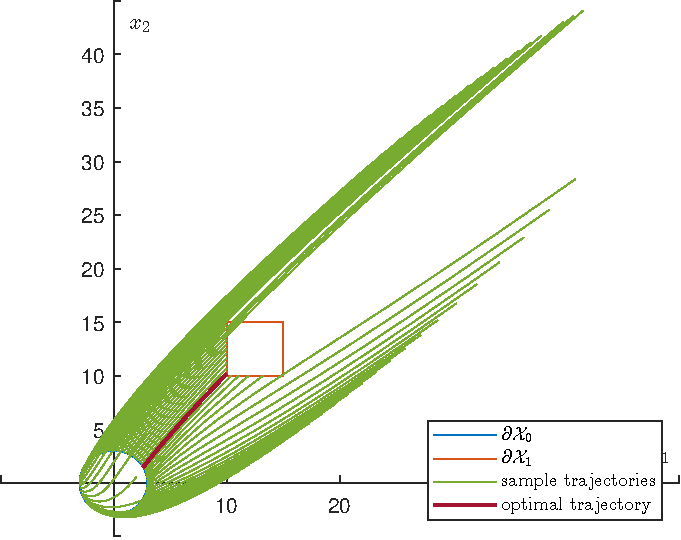
\includegraphics[width=0.6\textwidth]{examples/opt_traj_exmp3}
				\caption{Траектории подозрительные на оптимальность}
			\end{figure}
			\begin{figure}[h]
				\centering
				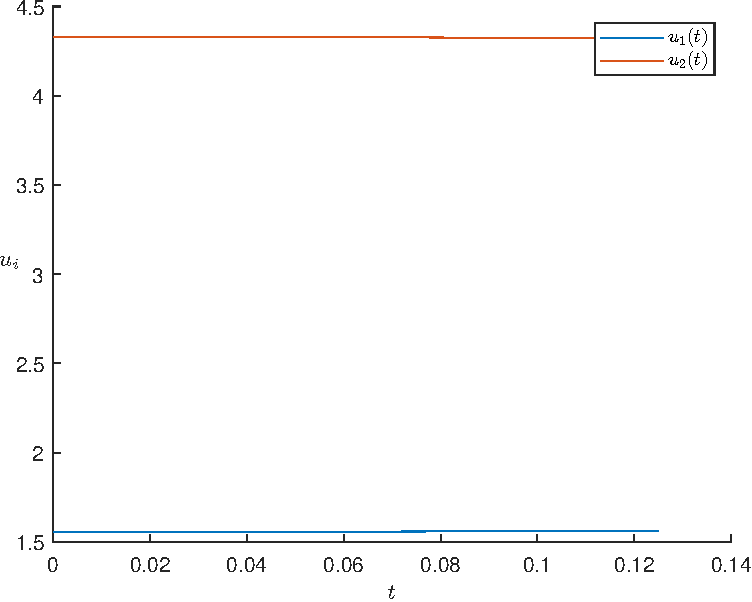
\includegraphics[width=0.6\textwidth]{examples/opt_cntrl_exmp3}
				\caption{Компоненты найденного приближенно-оптимального управления}
			\end{figure}
			\begin{figure}[h]
				\centering
				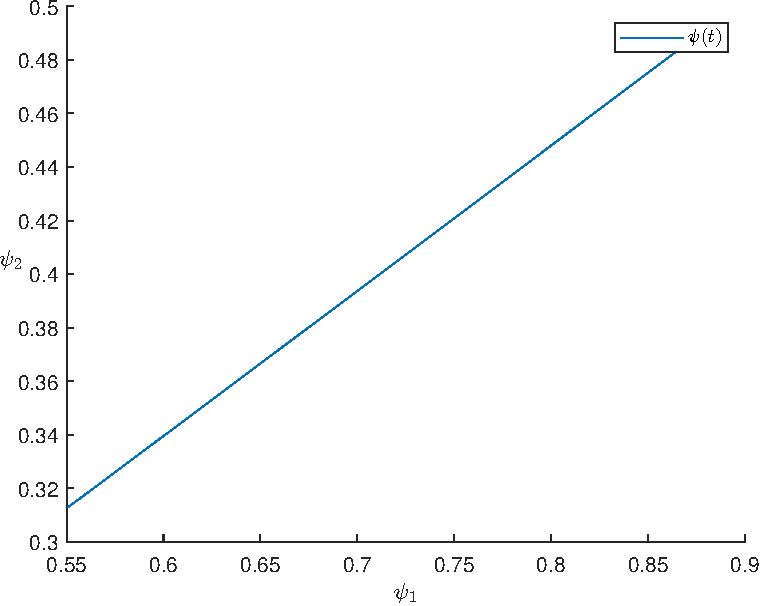
\includegraphics[width=0.6\textwidth]{examples/conj_exmp3}
				\caption{Сопряженная переменная}
			\end{figure}
Достигнутое время \(t^*_{min} \approx 0,126\); ошибка условия трансверсальности на правом конце \(\approx 0,049\).

		\subsection{неавтономная система}
			\begin{gather*}
				\confAB{\sin(t)}{2}{e^{-t}}{\cos(t)}{1}{e^{2t}}{t^3 + 2t -1}{t}
				\conffalphar{2t}{-t}{1}{2}{3}{3}{5}{3,5}
				\confq{12}{10}{10}{15}{15}{9}{17}{15}
			\end{gather*}
			\begin{figure}[h]
				\centering
				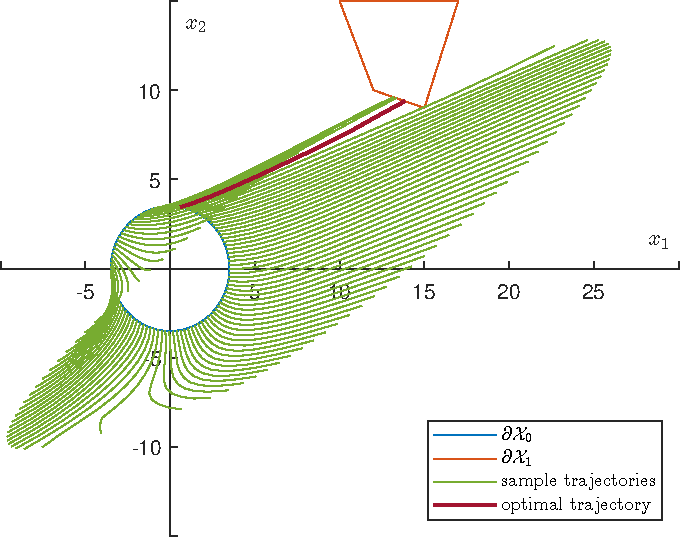
\includegraphics[width=0.6\textwidth]{examples/opt_traj_exmp1}
				\caption{Траектории подозрительные на оптимальность}
			\end{figure}
			\begin{figure}[h]
				\centering
				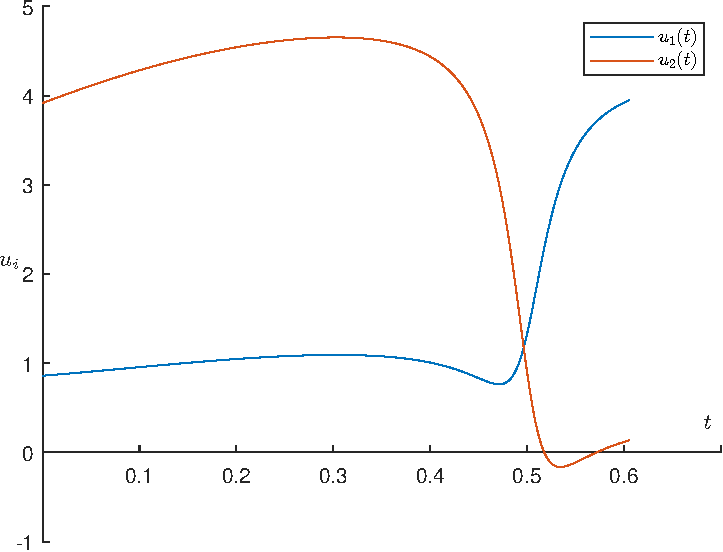
\includegraphics[width=0.6\textwidth]{examples/opt_cntrl_exmp1}
				\caption{Компоненты найденного приближенно-оптимального управления}
			\end{figure}
			\begin{figure}[h!]
				\centering
				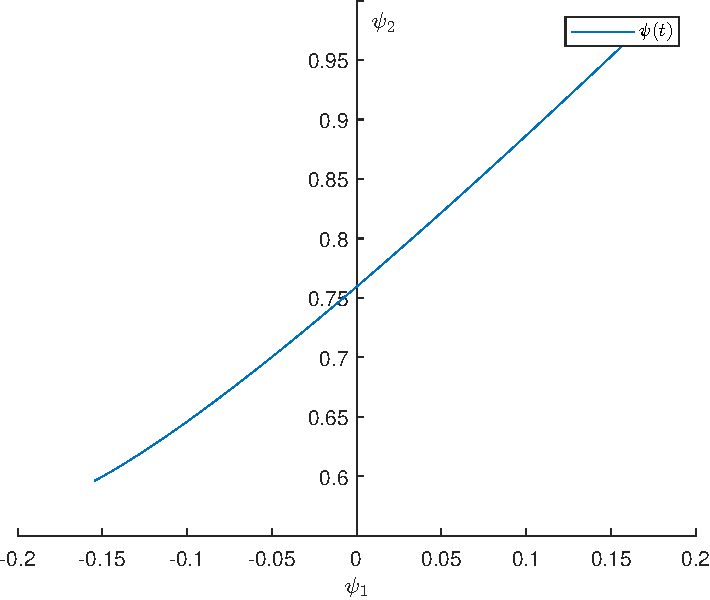
\includegraphics[width=0.6\textwidth]{examples/conj_exmp1}
				\caption{Сопряженная переменная}
			\end{figure}
Достигнутое время \(t^*_{min} \approx 0,607\); ошибка условия трансверсальности на правом конце \(\approx 0,406\).

		\subsection{отсутствие свойства непрерывности в поставленной задаче}
			\begin{gather*}
				\confAB{\sin(t)}{2}{e^{-t}}{\cos(t)}{1}{e^{2t}}{t^3 + 2t -1}{t}
				\conffalphar{2t}{-t}{1}{2}{3}{3}{5}{3,5}
				\confq{12}{12}{10}{17}{15}{11}{17}{17}
			\end{gather*}
			\begin{figure}[h]	
				\centering
				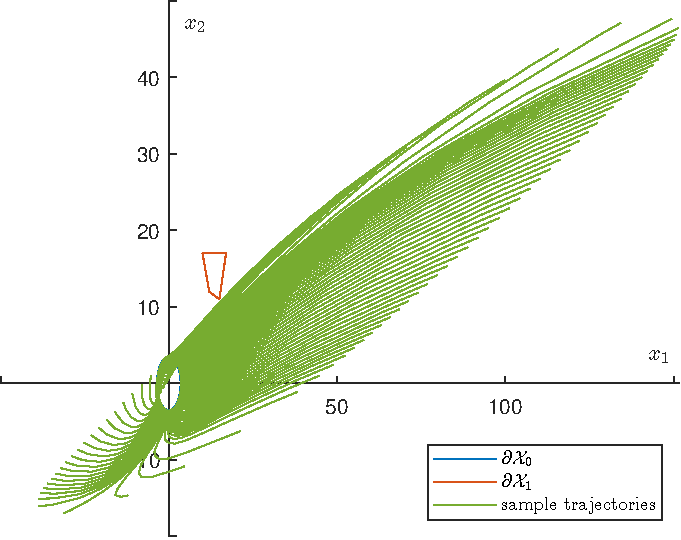
\includegraphics[width=0.6\textwidth]{examples/traj_exmp2}
				\caption{Траектории подозрительные на оптимальность (масштаб осей  отн. пр. 3.2 изменен)}
			\end{figure}
			
			В данном примере наглядно виден эффект отсутствия непрерывной зависимости минимального времени \(t^*_{min}\) от целевого множества. Параметры данной задачи идентичны предыдущей, за исключением лишь того, что целевое множество сдвинуто немного вверх. Уже при таком малом смещении решение задачи качественно меняется: множество \(\Chi_1\) становится в принципе недостижимым за обозримый промежуток времени.
	
	\begin{thebibliography}{0}
		\bibitem{PLF} Комаров~Ю.~А. кафедральный курс 
			\emph{"<Оптимальное управление (линейные системы)">}, 2020.
	\end{thebibliography}

\end{document}